	\section{Versuchsaufbau und -Durchführung \label{Aufbau}}
	
	\subsection{Eichung des MCA und Setzen des Energiefensters}\label{sec:eichung}
	
	Zu Beginn des Versuchs werden mit Hilfe verschiedener Metalle, deren Emissionsspektren bekannt sind, Eichmessungen durchgeführt. Dabei werden die Emissionsspektren aufgenommen und die bekannten Linien in diesen Spektren identifiziert. Anschließend wird daraus ein Umrechnungsfaktor zwischen Channels und Energie berechnet, und damit der zu beobachtende $14,4\,\si{keV}$-Peak von $^{57}\mathrm{Fe}$ identifiziert. Nun wird das Energiefenster des SCAs auf den $14.4\,\si{kev}$-Peak gesetzt, um nur Photonen mit dieser Energie zu detektieren. Zur Aufnahme der Eichspektren wird die in Abbildung \ref{fig:aufbaueich} beschriebene Schaltung verwendet.
	
	\begin{figure}[h!]
		\centering
		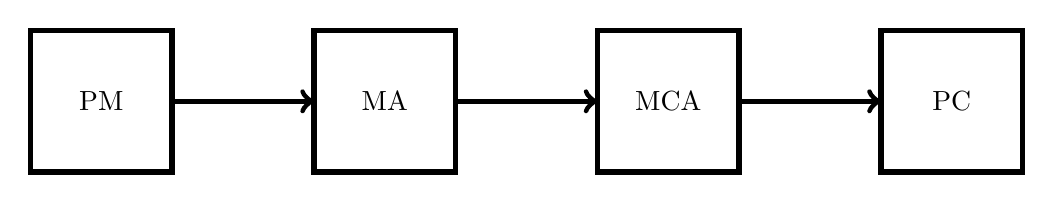
\begin{tikzpicture}[scale=0.9]
		\draw[line width=2] (-1,-1) rectangle (1,1);
		\draw[line width=2] (3,-1) rectangle (5,1);
		\draw[line width=2] (7,-1) rectangle (9,1);
		\draw[line width=2] (11,-1) rectangle (13,1);
		
		\draw[line width=2,->] (1,0) --(3,0);
		\draw[line width=2,->] (5,0) --(7,0);
		\draw[line width=2,->] (9,0) --(11,0);
		
		\node at (0,0) {PM};
		\node at (4,0) {MA};
		\node at (8,0) {MCA};
		\node at (12,0) {PC};
		
		
		\end{tikzpicture}
		\caption[Schematische Darstellung des Versuchsaufbaus für die Eichmessung]{Schematische Darstellung des Versuchsaufbaus für die Eichmessung}
		\label{fig:aufbaueich}
	\end{figure}

	\subsection{Aufbau der Schaltung}

	\begin{figure}[h!]
		\centering
		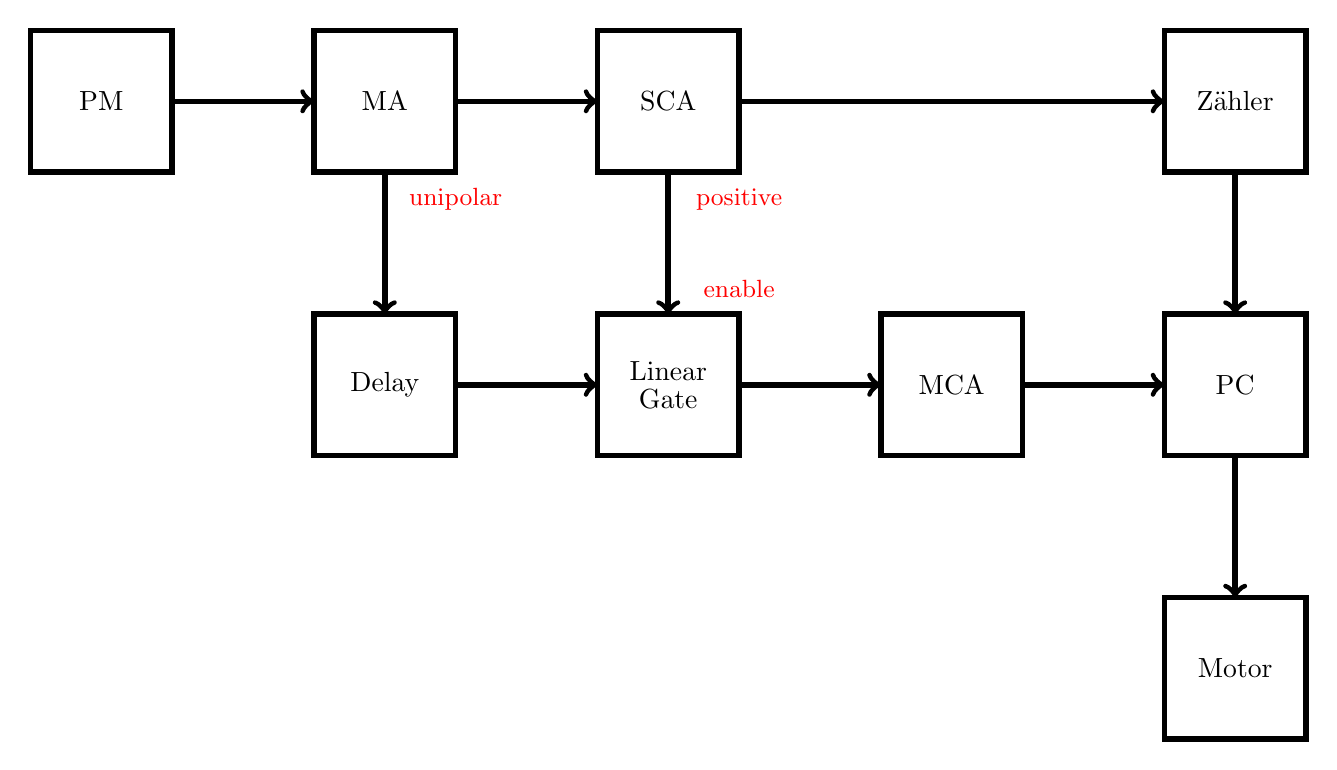
\begin{tikzpicture}[scale=0.9]
		\draw[line width=2] (-1,-1) rectangle (1,1);
		\draw[line width=2] (3,-1) rectangle (5,1);
		\draw[line width=2] (7,-1) rectangle (9,1);
		\draw[line width=2] (15,-1) rectangle (17,1);
		\draw[line width=2] (3,-5) rectangle (5,-3);
		\draw[line width=2] (7,-5) rectangle (9,-3);
		\draw[line width=2] (11,-5) rectangle (13,-3);
		\draw[line width=2] (15,-5) rectangle (17,-3);
		\draw[line width=2] (15,-7) rectangle (17,-9);
		
		\draw[line width=2,->] (1,0) --(3,0);
		\draw[line width=2,->] (5,0) --(7,0);
		\draw[line width=2,->] (9,0) --(15,0);
		\draw[line width=2,->] (5,-4) --(7,-4);
		\draw[line width=2,->] (9,-4) --(11,-4);
		\draw[line width=2,->] (13,-4) --(15,-4);
		\draw[line width=2,->] (4,-1) --(4,-3);
		\draw[line width=2,->] (8,-1) --(8,-3);
		\draw[line width=2,->] (16,-1) --(16,-3);
		\draw[line width=2,->] (16,-5) --(16,-7);
		
		\node at (0,0) {PM};
		\node at (4,0) {MA};
		\node at (8,0) {SCA};
		\node at (16,0) {Zähler};
		\node at (4,-4) {Delay};
		\node at (8,-3.8) {Linear};
		\node at (8,-4.2) {Gate};
		\node at (12,-4) {MCA};
		\node at (16,-4) {PC};
		\node at (16,-8) {Motor};
		
		\node[color=red,fill=white] at (5,-1.38) {\small unipolar};
		\node[color=red,fill=white] at (9,-1.38) {\small positive};
		\node[color=red,fill=white] at (9,-2.65) {\small enable};
		
		\end{tikzpicture}
		\caption[Schematische Darstellung des Versuchsaufbaus]{Schematische Darstellung des Versuchsaufbaus. Hierbei bezeichnet PM den Photomultiplier mit dem Szintillationszähler, MA den Hauptverstärker und SCA den Single Channel Analyzer.}
		\label{fig:aufbau2}
	\end{figure}
	
	Die Schaltung für den Rest des Versuchs wird gemäß Abbildung \ref{fig:aufbau2} aufgebaut. Der Photomultiplier wird an den Hauptverstärker angeschlossen. Dieser liefert sowohl an den SCA als auch an das Linear Gate ein unipolares Signal (siehe Abbildung \ref{fig:ma}), welches über eine Delay-Einheit verzögert werden kann. Im SCA kann nun ein Energiefenster gesetzt werden, mit welchem der Durchlass des Linear Gates gesteuert werden kann (siehe Abbildung \ref{fig:sca}). Gleichzeitig ist der SCA an einen Zähler angeschlossen, welcher mit dem Programm zur Motorsteuerung auf dem PC verbunden ist. Ebenso ist das Linear Gate über einen MCA an den PC angeschlossen.\\
	
	\graX{MA}{Signalausgänge des Hauptverstärkers}{Unipolarer (gelb) und bipolarer (blau) Ausgang des Hauptverstärkers.\label{fig:ma}}
	
	\graX{MA}{Signalausgänge des SCA und des Linear Gates}{Signalausgänge des SCA (gelb) und des Linear Gates (blau).\label{fig:sca}}
	
	\clearpage
	\subsection{Untergrundmessungen}
	
	Die Messungen der Transmission werden durch zwei Untergrundfaktoren beeinflusst. Dies sind die Compton-Streuung von höherenergetischen Photonen und die Abschwächung durch das Plexiglas der Absorberhaltungen. Um diese zu bestimmen wird die Transmission durch Plexiglas gemessen. Zur Messung des Compton-Untergrunds wird die Zählrate der Quelle mit Abschirmung durch Aluminiumplatten für verschiedene Plattendicken gemessen und daraus der Compton-Untergrund zur Dicke $d_0=0$ extrapoliert.
	
	\subsection{Hauptmessungen}
	
	Nun werden die beiden Hauptmessungen durchgeführt. In der ersten Hauptmessung wird das Transmissionsspektrum in Abhängigkeit der Geschwindigkeit von Edelstahl (Einlinienabsorber) aufgenommen. Dazu wird die Edelstahlprobe mit Hilfe eines Motors in Geschwindigkeiten von $-6\,\si{mms^{-1}}$ bis $6\,\si{mms^{-1}}$ in Schritten von $0.05\,\si{mms^{-1}}$ bewegt. Dabei wird an jedem Messpunkt eine Messzeit von $600\,\si{s}$ eingestellt.\\
	
	Anschließend wird das Transmissionsspektrum von Natureisen (Sechslinienabsorber) aufgenommen. Hierbei werden mit dem Motor Geschwindigkeiten von $-8\,\si{mms^{-1}}$ bis $8\,\si{mms^{-1}}$ in Abständen von $0,1\,\si{mms^{-1}}$ abgefahren. Auch hier wird an jedem Messpunkt $600\,\si{s}$ lang gemessen.
	
%	\begin{figure}[h!]
%		\centering
%		\begin{tikzpicture}[scale=0.9]
%		\draw[line width=2] (-1,-1) rectangle (1,1);
%		\draw[line width=2] (3,-1) rectangle (5,1);
%		\draw[line width=2] (7,-1) rectangle (9,1);
%		\draw[line width=2] (7,-5) rectangle (9,-3);
%		\draw[line width=2] (11,-5) rectangle (13,-3);
%		
%		\draw[line width=2,->] (1,0) --(3,0);
%		\draw[line width=2,->] (5,0) --(7,0);
%		\draw[line width=2,->] (4,-1) --(4,-4) --(7,-4);
%		\draw[line width=2,->] (9,-4) --(11,-4);
%		\draw[line width=2,->] (8,-1) --(8,-3);
%		
%		\node at (0,0) {PM};
%		\node at (4,0) {MA};
%		\node at (8,0) {SCA};
%		\node at (8,-3.8) {Linear};
%		\node at (8,-4.2) {Gate};
%		\node at (12,-4) {PC};
%		
%		\node[color=red,fill=white] at (5,-1.38) {\small unipolar};
%		\node[color=red,fill=white] at (9,-1.38) {\small positive};
%		\node[color=red,fill=white] at (9,-2.65) {\small enable};
%		
%		\end{tikzpicture}
%		\caption[Schematische Darstellung des Versuchsaufbaus zum Festlegen des Energiefensters]{Schematische Darstellung des Versuchsaufbaus zum Festlegen des Energiefensters}
%		\label{fig:aufbau}
%	\end{figure}
	
		
